Cloud part of this solution will be designed in a way to serve multi tenant and multi systems, using the same cloud resources.  Main principle of multi tenant system design is shown on figure \ref{fig:multi_tenant_simple}. One tenant f.e one factory will be able to have multiple systems on-site, where system means group of agents along the map-service and broker. To re-use some of tenants resources, systems will be also able to share the broker, what is shown in a details in appendix \ref{sec:app_03}.

\begin{figure}[H]
    \centering
    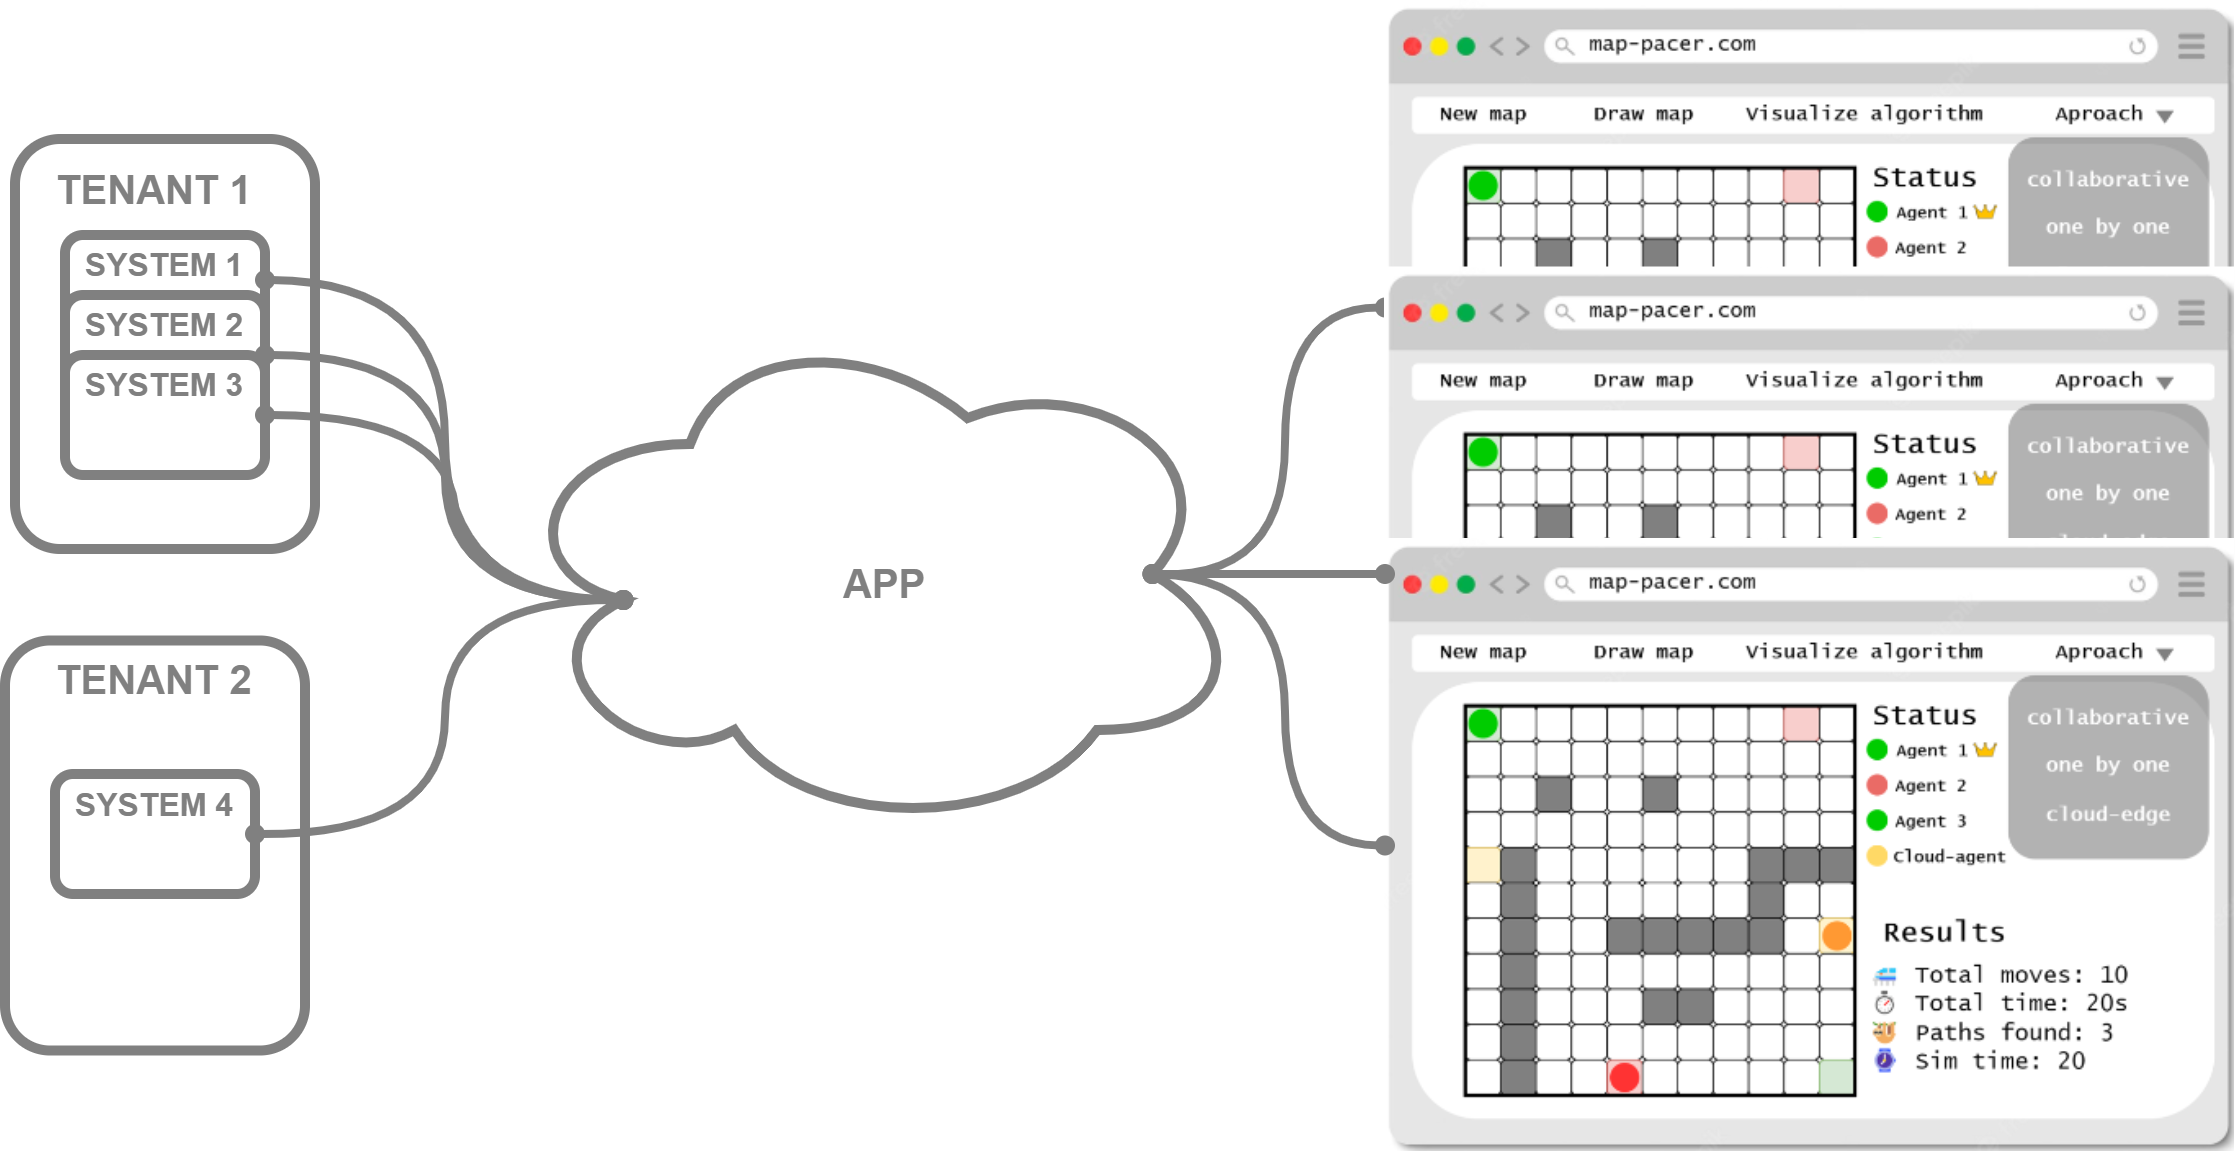
\includegraphics[width=\textwidth]{pictures/multi_tenant_simple.png}
    \caption{ Multi tenant system design }
    \label{fig:multi_tenant_simple}
\end{figure}


Cloud part of the solution will be shared among the tenants, and accessed through common web application. In final product, web application should expose logging page where tenant would provide credentials to authenticate himself. After successfully log in, tenant should have an option to choose the system which will be visualized. 

Cloud services should automatically scale when more and more tenants will be on boarded. Micro services should also be stateless with an exception of database, where all tenants data will be stored. Stateless services can easily be scaled horizontally, by auto-scaling, which would make system more flexible in case of scalability and flexibility.

